\documentclass[handout]{beamer}
%\documentclass{beamer}
\usetheme{Berlin}

\def\argmax{\mathop{\rm argmax}}
\def\argmin{\mathop{\rm argmin}}
\def\var{\mathop{\rm var}}
\def\cov{\mathop{\rm cov}}
\def\sign{\mathop{\rm sign}}
 \def\f{\mathop{\bf f}}
 \def\h{\mathop{\bf h}}
\usepackage{epsfig,amssymb,amsmath,enumerate,color,verbatim}
\usepackage{beamerthemesplit}
\usepackage{graphics}
\usepackage{graphicx}
\usepackage{hyperref}
\hypersetup{
    colorlinks=true,
    linkcolor=blue,
    filecolor=magenta,      
    urlcolor=cyan,
}



\newtheorem{ex}{Exercise}


\title[Boosting]{ Boosting}
\author[Xiang Zhou]{%
  Xiang Zhou}
  \institute[City University of Hong Kong]{%
  Department of Mathematics \\
  City University of Hong Kong\\
  Based on the slides of Junhui Wang}

\date[\today]{ 2019}
\subject{Statistics}

\begin{document}

\frame {

\titlepage

}



%%%--------------------------------------------------------------------



%%%--------------------------------------------------------------------

\frame {

\frametitle{Boosting}

\begin{itemize}
\item Iteratively learning weak classifiers
\item Final result is the weighted sum of the results of each weak classifiers
\item Many different boosting algorithms: adaboost (adaptive boosting) by  Freund and Schapire (1996) is the first.
\footnote{ In 2004, Yoav Freund and
\href{http://rob.schapire.net/}{ Rob Schapire}
won the 2003 Godel prize in Theoretical Computer Science  and the ACM's Paris Kanellakis Award for their 
AdaBoost in 2004, for theoretical accomplishments that
have had a significant and demonstrable effect on the practice of
computing.}
\item Examples of other boosting algorithms:
\begin{itemize}
\item LogitBoost (Friedman, Hastie and Tibshirani, AOS, 2000)
\item L2Boost (Buhlmann and Yu, JASA, 2002)
\item Others in machine learning community...
\end{itemize}
\item Focus on binary classification, and may be extended to multiclass case
\end{itemize}

}




%%%--------------------------------------------------------------------

\frame {

\frametitle{Adaboost.M1 algorithm}

Training data: $(x_i, y_i)$; $i=1,\ldots,n$ with $x_i \in  \mathbb{R}^p$ and $y_i \in \{-1,1\}$

\begin{enumerate}
\item Initialize $w_{1,i}=1/n$; $i=1,\ldots,n$
\item For $m=1$ to $M$:
\begin{enumerate}[a.]
\item Fit a weak classifier\footnote{
also called base learner. $h$ can take real values (``confidence-rated prediction'' by Shapire and Singer) and the 
classifier is then $\sign(h)$;  } $h_m(x):\mathbb{R}^p \rightarrow \{-1,1\}$ to the training data with weights $w_{m,i}$
\footnote{This means the loss function  is weighted:  $\min_{h_m}\sum_{i=1}^n  w_{m,i}\ell (x_i, h_m(x_i))$}
\item Compute weighted misclassification error:
\begin{equation}\label{em}
\epsilon_m=\sum_{i=1}^n w_{m,i} I(y_i \neq h_m(x_i))
\end{equation}
\item Compute \textcolor{red}{$\alpha_m = \frac{1}{2} \log( (1-\epsilon_m)/\epsilon_m )$}
\item Update \textcolor{red}{$w_{m+1,i}=w_{m,i} \exp(-y_i \alpha_m  h_m(x_i))/Z_m$}, where $Z_m=\sum_i w_{m,i} \exp(-y_i \alpha_m  h_m(x_i))$ is for normalization.
\end{enumerate}
\item Output $f(x)= \frac{\sum_m \alpha_m h_m(x)}{\sum_m \alpha_m}$ and $G(x)=\sign(f(x))$
\end{enumerate}

}



%%%--------------------------------------------------------------------

\frame {

\frametitle{Weak classifier and weights for sample population }

\begin{itemize}
\item The key parameters in Adaboost.M1 are the weights $\{w_i\}$ which are adaptively updated in each iteration:
\begin{block}
{The weight $w_i$ increases weights on misclassified points and decreases weights on correctly classified points.}
 \end{block}
 and $\{\alpha_m\}$  summing up all the contributions from each $h_m$: 
\begin{block}
{The weight $\alpha_m$  should be larger for the  weak classifiers $h_m$ with better performance (i.e. with 
the smaller $\epsilon_m$).  }
 \end{block}
 \item 
 But there are still infinite number of choices of these two sets of weight parameters.
 Why Adaboost takes this form?

\item Adaboost is \textcolor{red}{almost assumption free} except that $\alpha_m > 0$ or equivalently $\epsilon_m < 1/2$; i.e., the weak classifier needs to be better than ``random guessing" for any weights $w_{m,i}$.
\item The weak classifiers are often set as shallow
decision tree.
%\item Adaboost fits an additive model $\sum_m \alpha_m b(x;\gamma_m)$, where $b(x;\gamma_m)$'s are simple functions of $x$ characterized by parameters $\gamma_m$

\end{itemize}

}



%%%--------------------------------------------------------------------

\frame {

\frametitle{A simulated example}

\begin{figure}
\centering
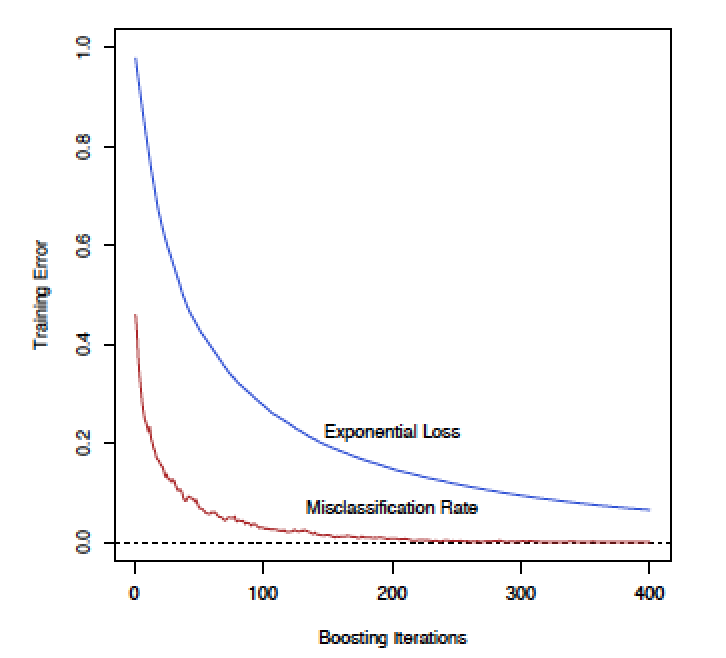
\includegraphics[width=3.in]{Chp10_3.jpeg}
\end{figure}

}


%%%--------------------------------------------------------------------

\frame {
\frametitle{ The recursive  idea     in boosting}
 
%
%\[ \log w_{m+1,i}= \log w_{m,i}   -\alpha_m  c_{m.i}\]
%which  $c_{m,i}$ should measure the training error of the classifier $h_m$ on the sample $(x_i, y_i)$.
%$y_i  h_m(x_i) $
%$\alpha_m$ should measure the all 
%

$$
\min_f L(f) = \sum_{i=1}^n \ell(y_i, f(x_i))
$$

\vspace{0.5cm}
The final classifier takes the additive form $f_M(x) = \sum_{m=1}^M \alpha_m h_m(x)$.
Consider the stagewise additive modeling \footnote{instead of considering all
terms $h_m$ and $\alpha_m$, $1\leq m\leq M$, simultaneously.}:
\begin{itemize}
\item Given $h_0(x),\ldots, h_{m-1}(x)$, how to find optimal $h_m$?
\item Compute the update as
$$
\boxed
{
(\alpha_m, h_m) = \argmin_{\alpha \in  \mathbb{R}^+,h \in {\cal H}} L(f_{m-1}+\alpha h)
}
\approx \sum_i \ell (y_i, f_m(x_i)+\alpha h(x_i)) 
$$
(Regularization can be added for $h$ by restricting $\cal H$)
\item Update $f_m(x) = f_{m-1}(x)+\alpha_m h_m(x)$, and then iterate.
\end{itemize}
 
}

 
%%%--------------------------------------------------------------------

\frame {

\frametitle{ Loss functions}
Recall
Table 12.1 in [ESL].
The loss function $\ell(y,f)$ usually takes the product form:
$\ell(y,f)= \ell(yf)$  for the binary classification.
\begin{itemize}
\item 0-1 loss: $\ell(y, f)=I(y \neq \sign(f))=\mbox{heaviside}(-yf)$
\begin{itemize}
\item Ideal but hard to work with (non-differentiable, discontinuous)
\end{itemize}


\item Binomial deviance: $\ell(y,f)=\log(1+\exp(-yf))$
\begin{itemize}
\item Fisher consistent; logistic regression
\end{itemize}
\item squared error: $(y-f)^2=(1-yf)^2$
\begin{itemize}
\item Not desirable as it penalizes correct classification
\end{itemize}
\item hinge loss: $(1-yf)_+$
\begin{itemize}
\item Fisher consistent; support vector machine 
\end{itemize}

\item exponential loss: $\exp(-yf)$

\begin{itemize}
\item Fisher consistent; large margin separation; Adaboost
\end{itemize}
\end{itemize}
The exponential function is very useful in our  
stagewise addition setting
since we are using the {\it additive} model now.

}


%%%--------------------------------------------------------------------

\frame {

\frametitle{ loss functions}

\begin{figure}
\centering
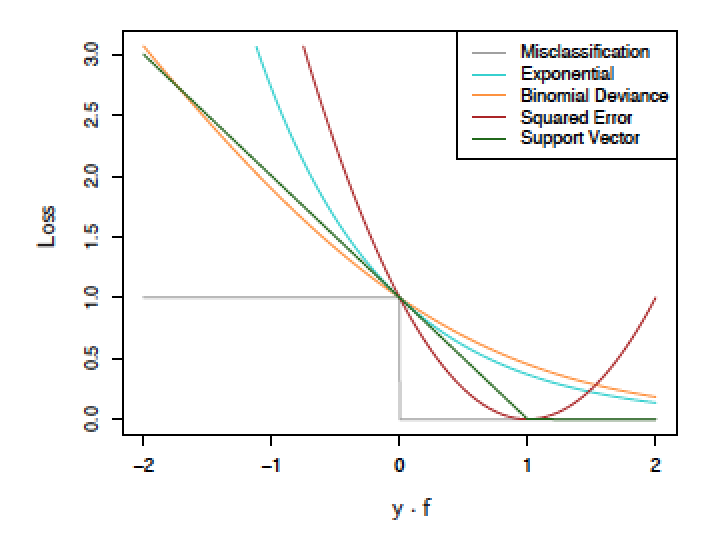
\includegraphics[width=3.3in]{Chp10_4.jpeg}
\end{figure}
Note: The 0-1 loss $\ell_{01}(y,f)=\mbox{heavisde}(-yf)$ is bounded from above by
the other loss $\ell(y,f)$. 
}




%%%--------------------------------------------------------------------

\frame {

\frametitle{AdaBoost: the magic of exponential loss  for additive model}

 

\begin{enumerate}
  \item The exponential loss function $
\ell(y,f(x)) = \exp (-yf(x))
$ is {\it Fisher consistent}:
$$
f^*=\argmin_f E(\exp(-Y f(X))) = \frac{1}{2} \log \frac{Pr(Y=1|X)}{1-Pr(Y=1|X)},
$$
and 
$
\sign(f^*(x)) = \sign(Pr(Y=1|X=x)-1/2)$  is the Bayes rule.
\item   The stagewise minimization for the additive model \begin{equation}\label{eq:adaboostloss}
\begin{split}
\min_{\alpha, h} \sum_{i=1}^n \exp(-y_i (f_{m-1}(x_i)+\alpha h(x_i))) 
\\
=\min_{\alpha, h} \sum_{i=1}^n w_i^{(m)} \exp(-\alpha y_i h(x_i))
\end{split}
\end{equation}
where $w_{i}^{(m)}=\exp(-y_i f_{m-1}(x_i)) $ equals  $w_{i}^{(m-1)} \exp(-y_i \alpha_{m-1}h_{m-1}(x_i)) $,
as  in  the Step 2.d of  AdaBoost.


\end{enumerate}
}


\frame{
\begin{itemize}

\item 
The exponential loss function 
is Fisher consistence, so 
 any $\alpha>0$, the weak learner $h_m $ is consistent with  the Bayes classifier:
  $\displaystyle h_m=\argmin_{h \in {\cal H}} \sum_i w_i^{(m)} I(y_i \neq h(x_i))$

\item Then  for given $h_m$,    \eqref{eq:adaboostloss} becomes the 
minimization for $\alpha$: 
 $$\min_\alpha \sum_{i=1}^n w_i^{(m)} \exp(-\alpha y_i h_m(x_i))
=\min_\alpha (1-\epsilon_m) e^{-\alpha}
+\epsilon_m e^{\alpha})$$
where the weighted misclassification rate $\epsilon_m$ is defined in \eqref{em}
gives 
 $\alpha_m = \frac{1}{2} \log( (1-\epsilon_m)/\epsilon_m )$,
 as in Step 2.c of AdaBoost.
\item The weal learner assumption: 
$$\alpha_m>0 \iff \epsilon_m >1/2
$$
\end{itemize}

}



%%%--------------------------------------------------------------------

\frame {

 
\begin{itemize}
\item
LogitBoost: apply the same idea to the 
log-loss function  used in logistic regression,
but with more complicated and less elegant computations.

\end{itemize}



}



%%%--------------------------------------------------------------------

\frame {{Boosting}
\[ (\alpha_m, h_m) = \argmin_{\alpha \in  \mathbb{R}^+,h \in {\cal H}} L(f_{m-1}+\alpha h)
\]
\begin{enumerate}
\item 
This is similar to the idea of coordinate descent for 
$\min_{\{\alpha_m, h_m: m=1,2,\ldots\} }
L(\sum_m \alpha_m f_m)$.
\item This stagewise addition has 
some implicit effect of regularization, since the 
search direction for $f$ is restricted to one component
each time.
\item Gradient boosting\footnote{Friedman, J. H. Greedy function approximation: a gradient
boosting machine. Ann. Statist., 29(5):1189–1232, 2001.
}
:
$h$ is set as the gradient of $L$ at $f_{m-1}$, or 
its projection in some restricted space $\cal H$.
\item $h$ does not have to be gradient:
it works as long as adding $h_m$ can decrease the loss function further.
\end{enumerate}


}


%%%--------------------------------------------------------------------

\frame {

\frametitle{Does boosting overfit? }

Boosting algorithms are relatively immune to overfitting but it does overfit slightly after a long time of iterations.
\vspace{-0.5cm}
\begin{figure}
\centering
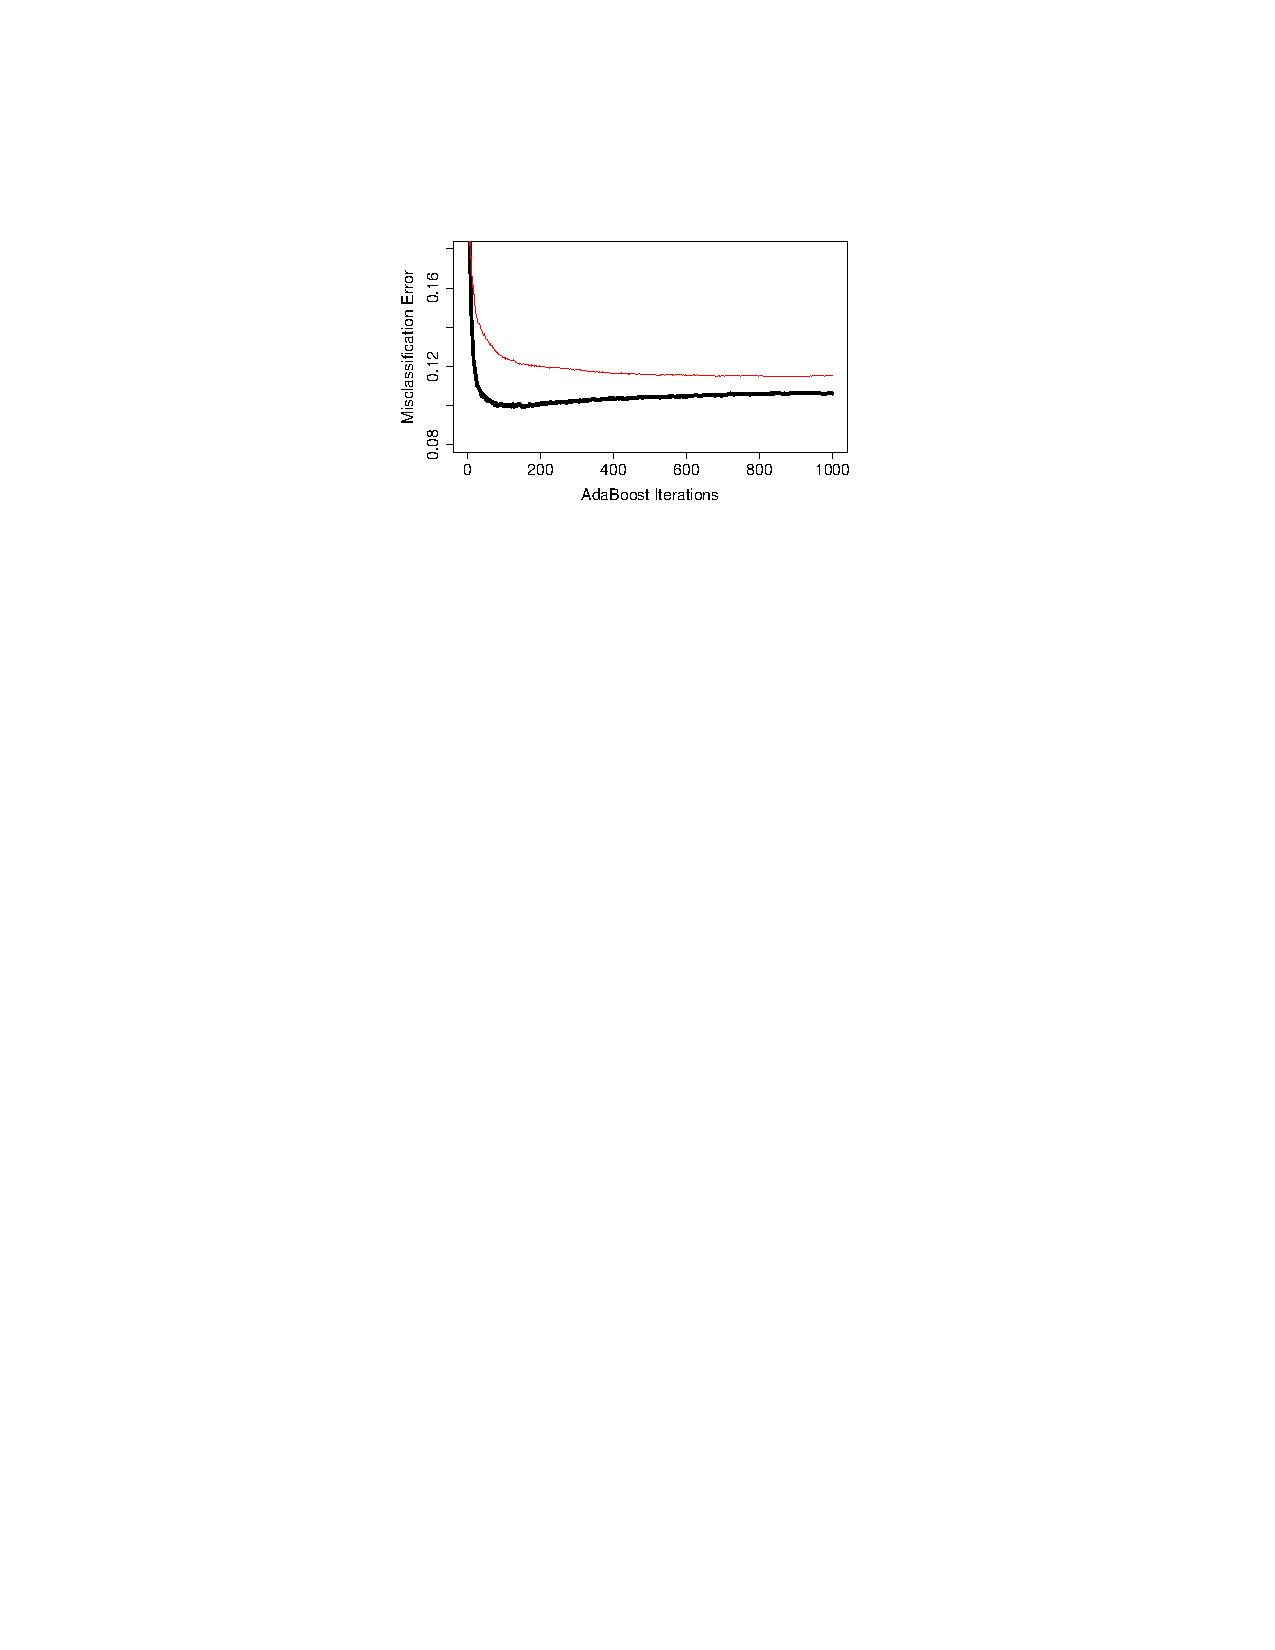
\includegraphics[width=3.5in]{Chp10_1.pdf}
\end{figure}
\vspace{-0.5cm}
Red line: Adaboost with 8-node trees; black line: Adaboost with stumps (one-node trees)

}



%%%--------------------------------------------------------------------

\frame {

\frametitle{Regularization}

\begin{itemize}
\item Early stopping (Zhang and Yu, 2005): stop the boosting algorithm at a medium number of iterations
\item Shrinkage (Lugosi and Vayatis, 2003):
$$
f_m(x) = f_{m-1}(x)+\nu \cdot \alpha_m h_m(x),
$$
where $0<\nu<1$ is a shrinkage factor
\item These two approaches operate in a similar fashion by controlling $\sum_m \alpha_m$: small value of $M$ and small value of $\nu$ result in small $\sum_m \alpha_m$ and large training error, and vice versa
\end{itemize}

}




%%%--------------------------------------------------------------------

\frame {{ Analyzing the training error}
The most basic theoretical property of AdaBoost concerns its ability to reduce the training error.
\begin{enumerate}
\item  The 0-1 loss is bounded by exponential loss: with $f=\sum_m \alpha_m h_m$
\begin{small}
\begin{eqnarray*}
\frac{1}{n} \sum_{i=1}^n \ell_{01}(y_i, f(x_i)) &\leq & \frac{1}{n} \sum_{i=1}^n \exp \left ( - y_i \sum_{m=1}^M \alpha_m h_m(x_i) \right ) 
\end{eqnarray*}
\end{small}

\item By $w_{m+1,i}=w_{m,i} \exp(-y_i \alpha_m  h_m(x_i))/Z_m$,
\begin{small}
\begin{eqnarray*}
& \frac{1}{n} \sum_{i=1}^n \exp \left ( - y_i \sum_{m=1}^M \alpha_m h_m(x_i) \right ) 
\leq 
 \frac{1}{n}  \sum_{i=1}^n  \prod_{m=1}^{M} \left(Z_m\frac{ w_{m+1,i} }{ w_{m,i}} \right)\\
 & =
 \frac{1}{n}  \sum_{i=1}^n  \left(\prod_{m=1}^{M} Z_m\right) \frac{w_{M+1,i}}{w_{1,i}}
 \\
 &= \left ( \prod_{m=1}^M Z_m \right ) \sum_{i=1}^n w_{M+1,i}=
\prod_{m=1}^M Z_m 
\end{eqnarray*}
\end{small}

\end{enumerate}


}

\frame{\begin{theorem}
The training error of the final classifier of the adaboost decays 
exponentially in the iteration number $M$:
\begin{align*}
 \frac{1}{n} \sum_{i=1}^n \ell_{01}(y_i, f(x_i))  \leq   \prod_{m=1}^M Z_m 
= \prod_{m=1}^M \sqrt{1-4\gamma_m^2}
\\
 \leq \exp(-2\sum_{m=1}^M \gamma_m^2)
\leq \exp(-2\gamma^2 M)
\end{align*}
where $\gamma_m = \epsilon_m -0.5$ and $\gamma=\min_m \gamma_m $.
\end{theorem}
The second line is a trivial consequence of the fact $\sqrt{1-t}\leq e^{-t/2}, t\in [0,1]$.
}
 
 
 
\frame {

\frametitle{Proof}

The last equality in the first line follows from
$$
w_{m+1,i}=\frac{w_{m,i} \exp(-y_i \alpha_m  h_m(x_i))}{Z_m}.
$$
Note that $\sum_{i=1}^n w_{M+1,i}=1$, $\alpha_m = \frac{1}{2} \log( (1-\epsilon_m)/\epsilon_m )$, and
\begin{eqnarray*}
Z_m &=& \sum_{i=1}^n w_{m,i} \exp(-y_i \alpha_m  h_m(x_i)) \\
&=& \sum_{\{i: y_i = h_m(x_i)\}} w_{m,i} e^{-\alpha_m} + \sum_{\{i: y_i \neq h_m(x_i)\}} w_{m,i} e^{\alpha_m} \\
&=& (1-\epsilon_m) e^{-\alpha_m} + \epsilon_m \alpha_m = 2 \sqrt{\epsilon_m (1-\epsilon_m)}.
\end{eqnarray*}
The desired upper bound is obtained after plugging in $\alpha_m$ and $Z_m$.

}


%%%--------------------------------------------------------------------

\frame {
The following exercise is a simple generalization of the above theorem.
 \begin{ex}
    For any $\theta>0$, show that
$$
\frac{1}{n} \sum_{i=1}^n I(y_i f(x_i) \leq \theta) \leq
\left ( \sqrt{(1-2\gamma)^{1-\theta} (1+2\gamma)^{1+\theta}} \right )^M,
$$
where the expression inside parenthesis $< 1$ when $\theta < \gamma$. 
 \end{ex}

}



%%%--------------------------------------------------------------------
%
%\frame {
%
%\frametitle{Proof}
%
%Note $y_i f(x_i) \leq \theta$ implies $y_i \sum_m \alpha_m h_m(x_i) \leq \theta \sum_m \alpha_m$ and
%$$
%\exp \left ( - y_i \sum_m \alpha_m h_m(x_i) + \theta \sum_m \alpha_m \right ) \geq 1.
%$$
%\begin{small}
%\begin{eqnarray*}
%\frac{1}{n} \sum_{i=1}^n I(y_i f(x_i) \leq \theta) &\leq & \frac{1}{n} \sum_{i=1}^n \exp \left ( - y_i \sum_m \alpha_m h_m(x_i) + \theta \sum_m \alpha_m \right ) \\
%&=& \exp(\theta \sum_m \alpha_m) \frac{1}{n} \sum_{i=1}^n \exp \left ( - y_i \sum_m \alpha_m h_m(x_i) \right ) \\
%&=& \exp \left (\theta \sum_m \alpha_m \right ) \left ( \prod_{m=1}^M Z_m \right ) \sum_{i=1}^n w_{M+1,i}
%\end{eqnarray*}
%\end{small}
%
%}



%%%--------------------------------------------------------------------





\frame{{Generalization Error}

The generalization error is bounded by  for any positive $\theta$
\[
 {\Pr}_{\cal D} \left( Yf(X) \leq \theta \sum_{m=1}^M |\alpha_m| \right)
+ O(\sqrt{\frac{d}{n \theta^2}})
\]
where $d$  is the VC dimension of the hypothesis space $\mathcal{H}$
and $n$ is the number of training samples. 
$\Pr_{\cal D}$ is the prob. w.r.t. the training data.

The second term is independent of the iteration number $M$.
\bigskip
Ref:
{\tiny
Robert E. Schapire, Yoav Freund, Peter Bartlett, and Wee Sun Lee. Boosting the margin: A new explanation for the effectiveness of voting methods. The Annals of Statistics, 26(5):1651–1686, October 1998.
}
}




%%%--------------------------------------------------------------------

\frame {

\frametitle{Example: L2Boost}
$$
L(f) = \frac{1}{2} \sum_{i=1}^n (y_i - f(x_i))^2
$$
\begin{itemize}
\item Initialize $f_0(x)=\bar y$
\item Compute $g_m(x_i) = y_i-f_{m-1}(x_i)=r_i$
\item Compute $(\alpha_m,h_m) = \argmin_{\alpha, h \in {\cal H}} \sum_{i=1}^n (r_i- \alpha h(x_i))^2$
\item Update $f_m(x) = f_{m-1}(x)+\alpha_m h_m(x)$, and iterate
\end{itemize}

\vspace{0.5cm}
Remarks: This boils down to the standard approach of iteratively fitting the residuals

}

%%%--------------------------------------------------------------------

\frame {

\frametitle{Example: LogitBoost}

$$
L(f) = \sum_{i=1}^n \log(1+\exp(-2y_if(x_i)))
$$
\begin{itemize}
\item Initialize $f_0(x)=\frac{1}{2} \log \frac{1+\bar y}{1-\bar y}$
\item Compute the gradient at $f_{m-1}$: $g_m(x_i) = 2y_i/(1+\exp(2y_if_{m-1}(x_i))) = \tilde y_i$
\item Compute $h_m = \argmax_{h \in {\cal H}}~\sum_{i=1}^n \tilde y_i h(x_i)$
\item Approximate $\alpha_m$ by a Newton-Raphson step
\item Update $f_m(x) = f_{m-1}(x)+\alpha_m h_m(x)$, and iterate
\end{itemize}

 
}

%%%--------------------------------------------------------------------


%%%--------------------------------------------------------------------

\frame {

\frametitle{Multiclass boosting}

Training sample $(x_i,y_i)_{i=1}^n$ with $x_i \in \mathcal{R}^p$ and $y_i \in \{1,\ldots,K\}$. Denote $\f=(f_1,\ldots,f_K)^T$ and $G(x)=\argmax_k f_k(x)$.

\begin{itemize}
\item Generalization error: $GE(\f)=P(Y \neq G(X))$
\item Bayes rule: $G^*(x) = \argmax_k Pr(Y=k|X=x)$
\item Sum-to-zero constraint: $\sum_k f_k(x) =0$ for all $x$
\end{itemize}

}




%%%--------------------------------------------------------------------

\frame {

\frametitle{Multiclass loss function}

Various multiclass loss functions $L(y,\f)$ are proposed:
\begin{itemize}
\item $\sum_{k \neq y} \exp (f_k(x)-f_y(x))$ (Schapire and Singer, 1999)
\item $\sum_{k \neq y} f_k^q (x)$ (Lozano and Abe, 2008)
\item $\exp(-\frac{f_y(x)}{K-1})$ (Zhu et al., 2009)
\item $\sum_{k \neq y} \exp (f_k(x))$ (Wang, 2011)
\end{itemize}

}




\frame{{Further Readings}


Boosting  is argued to be  one of the
most successful practical tools
arising from theoretic machine learning.
One successful applications include the human face recognition, the spam filters.
There are a few great theories 
on adaboost we did not cover here.

\bigskip

\href{http://rob.schapire.net/papers/explaining-adaboost.pdf}{Explaining AdaBoost by 
Robert E. Schapire
}
\bigskip

\href{http://www.cs.princeton.edu/courses/archive/spr07/cos424/papers/boosting-survey.pdf}{An overview of Boosting Approach}

\bigskip
Book:
Boosting: Foundations and Algorithms
by by Robert E. Schapire  and  Yoav Freund (2012)

}

%%%--------------------------------------------------------------------
  \end{document}
